\hypertarget{main_8cpp}{
\section{main.cpp File Reference}
\label{main_8cpp}\index{main.cpp@{main.cpp}}
}
{\tt \#include $<$qapplication.h$>$}\par
{\tt \#include \char`\"{}tabs.h\char`\"{}}\par
{\tt \#include \char`\"{}database.h\char`\"{}}\par
{\tt \#include \char`\"{}printer.h\char`\"{}}\par
{\tt \#include \char`\"{}settings.h\char`\"{}}\par


Include dependency graph for main.cpp:\begin{figure}[H]
\begin{center}
\leavevmode
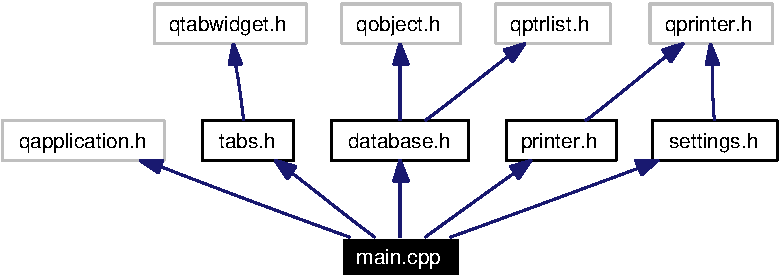
\includegraphics[width=204pt]{main_8cpp__incl}
\end{center}
\end{figure}
\subsection*{Functions}
\begin{CompactItemize}
\item 
int \hyperlink{main_8cpp_a0}{main} (int argc, char $\ast$argv\mbox{[}$\,$\mbox{]})
\end{CompactItemize}


\subsection{Function Documentation}
\hypertarget{main_8cpp_a0}{
\index{main.cpp@{main.cpp}!main@{main}}
\index{main@{main}!main.cpp@{main.cpp}}
\subsubsection[main]{\setlength{\rightskip}{0pt plus 5cm}int main (int {\em argc}, char $\ast$ {\em argv}\mbox{[}$\,$\mbox{]})}}
\label{main_8cpp_a0}


Definition at line 8 of file main.cpp.

References Settings::destroy(), Printer::destroy(), Database::destroy(), Printer::instance(), Database::instance(), and Settings::instance().

\footnotesize\begin{verbatim}9 {
10     QApplication app(argc,argv);
11     
12     Settings *settings = Settings::instance();
13     Database *db = Database::instance();
14     Printer *printer = Printer::instance();
15     
16     Tabs tabs(&app);
17     tabs.show();
18     app.setMainWidget(&tabs);
19     int retVal = app.exec();
20     db->destroy();
21     printer->destroy();
22     settings->destroy();
23     return retVal;
24 }
\end{verbatim}\normalsize 


